\documentclass[../slides.tex]{subfiles}
\begin{document}

\begin{frame}{Gliederung}
    \begin{block}{Themen}
        \begin{itemize}
            \item Addtive Fertigung
            \item Digitalisierung von Bauteilen
            \item Optische Spannkraftdeformationsanalyse
            \item Automatisierung
            \item Vergleich Herstellungsverfahren
            \item Zeitplan
        \end{itemize}
      \end{block}
\end{frame}

\begin{frame}{Additive Fertigung: Überblick}
  \begin{minipage}[t]{.40\textwidth}
    \begin{itemize}[]
      \item Marktwachstum von 18.3\%
      \item viele Anwendungsbereiche
    \end{itemize}  
  \end{minipage}
  \hfill
  \begin{minipage}[t]{.59\textwidth}
    \begin{figure}[]
      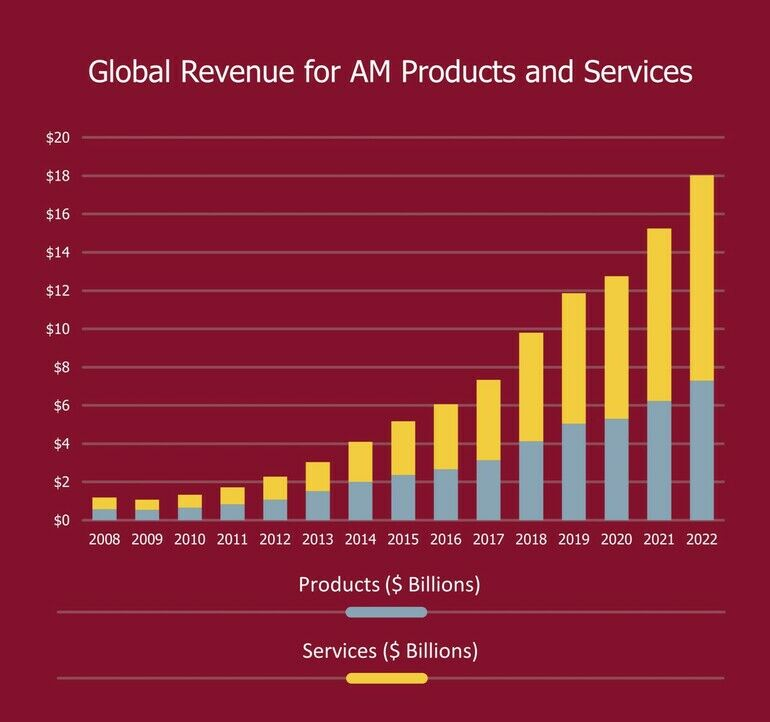
\includegraphics[height=165pt]{img_niklas/Picture3-1-scaled_0FB63A00-D319-40EF-A648-9739A68215D6.jpg}
      \caption[short]{Global Revenue for additive manufactured products}
      %https://additive.industrie.de/news/wohlers-report-2023-additive-fertigung-legt-um-183-zu/
    \end{figure}
  \end{minipage}
\end{frame}

\begin{frame}{Additive Fertigung: Verfahren}
  \begin{minipage}[t]{\textwidth}
    \begin{figure}[]
      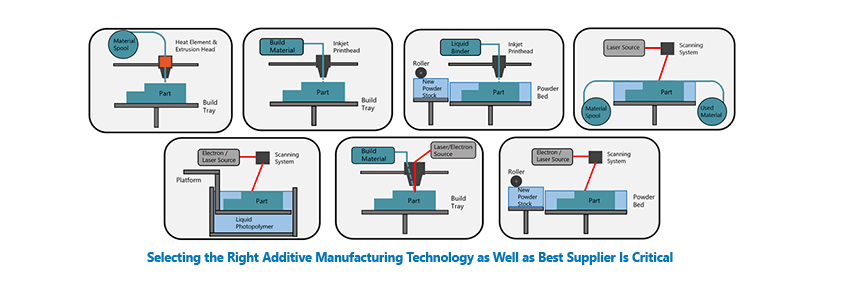
\includegraphics[width=\textwidth]{img_niklas/selecting-additive-manufacturing-technology-sm.png}
      \caption[short]{Additive Manufacturing System Selection Guide Overview}
      %https://www.arcweb.com/technology-evaluation-and-selection/additive-manufacturing-system-selection
    \end{figure}
  \end{minipage}
\end{frame}

\begin{frame}{Additive Fertigung: Limitierungen und Post-Processing}
  \begin{minipage}[t]{\textwidth}
    \begin{figure}[]
      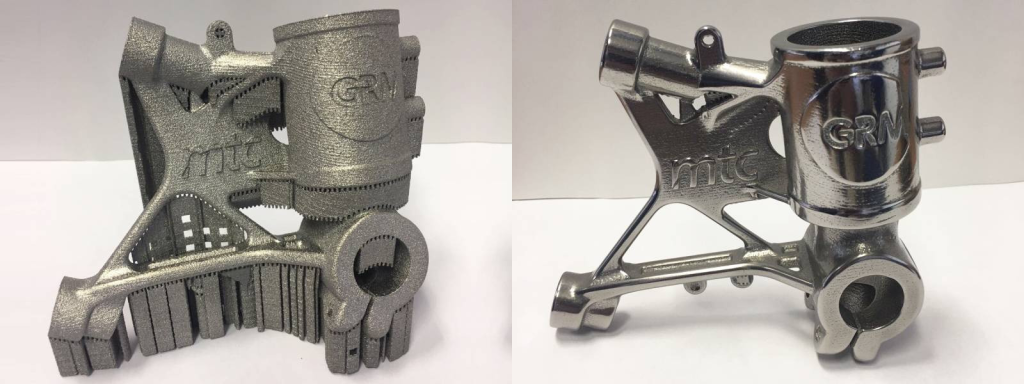
\includegraphics[width=\textwidth]{img_niklas/image-32-1024x384.png}
      \label{fig:meine-grafik}
      \caption[short]{Metal part post-processing: before and after}
      %https://www.unionfab.com/blog/2023/08/post-processing-methods-metal-3d-printing
    \end{figure}
  \end{minipage}
\end{frame}

\begin{frame}{Deformation durch einspannen}
  \begin{minipage}[h]{.40\textwidth}
    \begin{figure}[]
      
\includegraphics[height=150pt]{img_niklas/before_clamping.png}
      \caption[short]{Vor dem einspannen}
      %
    \end{figure}
  \end{minipage}
  \hfill
  \begin{minipage}[h]{.40\textwidth}
    \begin{figure}[]
      
\includegraphics[height=150pt]{img_niklas/after_clamping.png}
      \caption[short]{Nach dem einspannen}
      %
    \end{figure}
  \end{minipage}
\end{frame}



\end{document}